% Options for packages loaded elsewhere
\PassOptionsToPackage{unicode}{hyperref}
\PassOptionsToPackage{hyphens}{url}
%
\documentclass[
]{article}
\usepackage{lmodern}
\usepackage{amssymb,amsmath}
\usepackage{ifxetex,ifluatex}
\ifnum 0\ifxetex 1\fi\ifluatex 1\fi=0 % if pdftex
  \usepackage[T1]{fontenc}
  \usepackage[utf8]{inputenc}
  \usepackage{textcomp} % provide euro and other symbols
\else % if luatex or xetex
  \usepackage{unicode-math}
  \defaultfontfeatures{Scale=MatchLowercase}
  \defaultfontfeatures[\rmfamily]{Ligatures=TeX,Scale=1}
\fi
% Use upquote if available, for straight quotes in verbatim environments
\IfFileExists{upquote.sty}{\usepackage{upquote}}{}
\IfFileExists{microtype.sty}{% use microtype if available
  \usepackage[]{microtype}
  \UseMicrotypeSet[protrusion]{basicmath} % disable protrusion for tt fonts
}{}
\makeatletter
\@ifundefined{KOMAClassName}{% if non-KOMA class
  \IfFileExists{parskip.sty}{%
    \usepackage{parskip}
  }{% else
    \setlength{\parindent}{0pt}
    \setlength{\parskip}{6pt plus 2pt minus 1pt}}
}{% if KOMA class
  \KOMAoptions{parskip=half}}
\makeatother
\usepackage{xcolor}
\IfFileExists{xurl.sty}{\usepackage{xurl}}{} % add URL line breaks if available
\IfFileExists{bookmark.sty}{\usepackage{bookmark}}{\usepackage{hyperref}}
\hypersetup{
  pdftitle={Weekly chart data analysis},
  pdfauthor={Gregor Aisch},
  hidelinks,
  pdfcreator={LaTeX via pandoc}}
\urlstyle{same} % disable monospaced font for URLs
\usepackage[margin=1in]{geometry}
\usepackage{color}
\usepackage{fancyvrb}
\newcommand{\VerbBar}{|}
\newcommand{\VERB}{\Verb[commandchars=\\\{\}]}
\DefineVerbatimEnvironment{Highlighting}{Verbatim}{commandchars=\\\{\}}
% Add ',fontsize=\small' for more characters per line
\usepackage{framed}
\definecolor{shadecolor}{RGB}{248,248,248}
\newenvironment{Shaded}{\begin{snugshade}}{\end{snugshade}}
\newcommand{\AlertTok}[1]{\textcolor[rgb]{0.94,0.16,0.16}{#1}}
\newcommand{\AnnotationTok}[1]{\textcolor[rgb]{0.56,0.35,0.01}{\textbf{\textit{#1}}}}
\newcommand{\AttributeTok}[1]{\textcolor[rgb]{0.77,0.63,0.00}{#1}}
\newcommand{\BaseNTok}[1]{\textcolor[rgb]{0.00,0.00,0.81}{#1}}
\newcommand{\BuiltInTok}[1]{#1}
\newcommand{\CharTok}[1]{\textcolor[rgb]{0.31,0.60,0.02}{#1}}
\newcommand{\CommentTok}[1]{\textcolor[rgb]{0.56,0.35,0.01}{\textit{#1}}}
\newcommand{\CommentVarTok}[1]{\textcolor[rgb]{0.56,0.35,0.01}{\textbf{\textit{#1}}}}
\newcommand{\ConstantTok}[1]{\textcolor[rgb]{0.00,0.00,0.00}{#1}}
\newcommand{\ControlFlowTok}[1]{\textcolor[rgb]{0.13,0.29,0.53}{\textbf{#1}}}
\newcommand{\DataTypeTok}[1]{\textcolor[rgb]{0.13,0.29,0.53}{#1}}
\newcommand{\DecValTok}[1]{\textcolor[rgb]{0.00,0.00,0.81}{#1}}
\newcommand{\DocumentationTok}[1]{\textcolor[rgb]{0.56,0.35,0.01}{\textbf{\textit{#1}}}}
\newcommand{\ErrorTok}[1]{\textcolor[rgb]{0.64,0.00,0.00}{\textbf{#1}}}
\newcommand{\ExtensionTok}[1]{#1}
\newcommand{\FloatTok}[1]{\textcolor[rgb]{0.00,0.00,0.81}{#1}}
\newcommand{\FunctionTok}[1]{\textcolor[rgb]{0.00,0.00,0.00}{#1}}
\newcommand{\ImportTok}[1]{#1}
\newcommand{\InformationTok}[1]{\textcolor[rgb]{0.56,0.35,0.01}{\textbf{\textit{#1}}}}
\newcommand{\KeywordTok}[1]{\textcolor[rgb]{0.13,0.29,0.53}{\textbf{#1}}}
\newcommand{\NormalTok}[1]{#1}
\newcommand{\OperatorTok}[1]{\textcolor[rgb]{0.81,0.36,0.00}{\textbf{#1}}}
\newcommand{\OtherTok}[1]{\textcolor[rgb]{0.56,0.35,0.01}{#1}}
\newcommand{\PreprocessorTok}[1]{\textcolor[rgb]{0.56,0.35,0.01}{\textit{#1}}}
\newcommand{\RegionMarkerTok}[1]{#1}
\newcommand{\SpecialCharTok}[1]{\textcolor[rgb]{0.00,0.00,0.00}{#1}}
\newcommand{\SpecialStringTok}[1]{\textcolor[rgb]{0.31,0.60,0.02}{#1}}
\newcommand{\StringTok}[1]{\textcolor[rgb]{0.31,0.60,0.02}{#1}}
\newcommand{\VariableTok}[1]{\textcolor[rgb]{0.00,0.00,0.00}{#1}}
\newcommand{\VerbatimStringTok}[1]{\textcolor[rgb]{0.31,0.60,0.02}{#1}}
\newcommand{\WarningTok}[1]{\textcolor[rgb]{0.56,0.35,0.01}{\textbf{\textit{#1}}}}
\usepackage{graphicx,grffile}
\makeatletter
\def\maxwidth{\ifdim\Gin@nat@width>\linewidth\linewidth\else\Gin@nat@width\fi}
\def\maxheight{\ifdim\Gin@nat@height>\textheight\textheight\else\Gin@nat@height\fi}
\makeatother
% Scale images if necessary, so that they will not overflow the page
% margins by default, and it is still possible to overwrite the defaults
% using explicit options in \includegraphics[width, height, ...]{}
\setkeys{Gin}{width=\maxwidth,height=\maxheight,keepaspectratio}
% Set default figure placement to htbp
\makeatletter
\def\fps@figure{htbp}
\makeatother
\setlength{\emergencystretch}{3em} % prevent overfull lines
\providecommand{\tightlist}{%
  \setlength{\itemsep}{0pt}\setlength{\parskip}{0pt}}
\setcounter{secnumdepth}{-\maxdimen} % remove section numbering

\title{Weekly chart data analysis}
\author{Gregor Aisch}
\date{9/22/2020}

\begin{document}
\maketitle

\hypertarget{r-markdown}{%
\subsection{R Markdown}\label{r-markdown}}

Load some useful packages using \texttt{needs}

\begin{Shaded}
\begin{Highlighting}[]
\KeywordTok{needs}\NormalTok{(tidyverse, directlabels, ggrepel)}
\end{Highlighting}
\end{Shaded}

Let's load yearly, seasonal and monthly averages for air temperature

\begin{Shaded}
\begin{Highlighting}[]
\NormalTok{temp <-}\StringTok{ }\KeywordTok{read_delim}\NormalTok{(}\StringTok{'https://opendata.dwd.de/climate_environment/CDC/regional_averages_DE/annual/air_temperature_mean/regional_averages_tm_year.txt'}\NormalTok{,}
                   \DataTypeTok{delim=}\StringTok{';'}\NormalTok{, }\DataTypeTok{skip =} \DecValTok{1}\NormalTok{) }\OperatorTok\StringTok{ }
\StringTok{  }\KeywordTok{transmute}\NormalTok{(}\DataTypeTok{year=}\NormalTok{Jahr, }\DataTypeTok{time=}\StringTok{'Year'}\NormalTok{, }\DataTypeTok{value=}\KeywordTok{as.numeric}\NormalTok{(Deutschland)) }\OperatorTok\StringTok{ }
\StringTok{  }\KeywordTok{bind_rows}\NormalTok{(}
    \KeywordTok{read_delim}\NormalTok{(}\StringTok{'https://opendata.dwd.de/climate_environment/CDC/regional_averages_DE/seasonal/air_temperature_mean/regional_averages_tm_autumn.txt'}\NormalTok{,}
               \DataTypeTok{delim=}\StringTok{';'}\NormalTok{, }\DataTypeTok{skip =} \DecValTok{1}\NormalTok{) }\OperatorTok\StringTok{ }
\StringTok{      }\KeywordTok{transmute}\NormalTok{(}\DataTypeTok{year=}\NormalTok{Jahr,}\DataTypeTok{time=}\StringTok{'Autumn'}\NormalTok{, }\DataTypeTok{value=}\KeywordTok{as.numeric}\NormalTok{(Deutschland)),}
    \KeywordTok{read_delim}\NormalTok{(}\StringTok{'https://opendata.dwd.de/climate_environment/CDC/regional_averages_DE/seasonal/air_temperature_mean/regional_averages_tm_spring.txt'}\NormalTok{,}
               \DataTypeTok{delim=}\StringTok{';'}\NormalTok{, }\DataTypeTok{skip =} \DecValTok{1}\NormalTok{) }\OperatorTok\StringTok{ }
\StringTok{      }\KeywordTok{transmute}\NormalTok{(}\DataTypeTok{year=}\NormalTok{Jahr,}\DataTypeTok{time=}\StringTok{'Spring'}\NormalTok{, }\DataTypeTok{value=}\KeywordTok{as.numeric}\NormalTok{(Deutschland)),}
    \KeywordTok{read_delim}\NormalTok{(}\StringTok{'https://opendata.dwd.de/climate_environment/CDC/regional_averages_DE/seasonal/air_temperature_mean/regional_averages_tm_summer.txt'}\NormalTok{,}
               \DataTypeTok{delim=}\StringTok{';'}\NormalTok{, }\DataTypeTok{skip =} \DecValTok{1}\NormalTok{) }\OperatorTok\StringTok{ }
\StringTok{      }\KeywordTok{transmute}\NormalTok{(}\DataTypeTok{year=}\NormalTok{Jahr,}\DataTypeTok{time=}\StringTok{'Summer'}\NormalTok{, }\DataTypeTok{value=}\KeywordTok{as.numeric}\NormalTok{(Deutschland)),}
    \KeywordTok{read_delim}\NormalTok{(}\StringTok{'https://opendata.dwd.de/climate_environment/CDC/regional_averages_DE/seasonal/air_temperature_mean/regional_averages_tm_winter.txt'}\NormalTok{,}
               \DataTypeTok{delim=}\StringTok{';'}\NormalTok{, }\DataTypeTok{skip =} \DecValTok{1}\NormalTok{) }\OperatorTok\StringTok{ }
\StringTok{      }\KeywordTok{transmute}\NormalTok{(}\DataTypeTok{year=}\NormalTok{Jahr,}\DataTypeTok{time=}\StringTok{'Winter'}\NormalTok{, }\DataTypeTok{value=}\KeywordTok{as.numeric}\NormalTok{(Deutschland)),}
    \KeywordTok{read_delim}\NormalTok{(}\StringTok{'https://opendata.dwd.de/climate_environment/CDC/regional_averages_DE/monthly/air_temperature_mean/regional_averages_tm_01.txt'}\NormalTok{,}
               \DataTypeTok{delim=}\StringTok{';'}\NormalTok{, }\DataTypeTok{skip =} \DecValTok{1}\NormalTok{) }\OperatorTok\StringTok{ }
\StringTok{      }\KeywordTok{transmute}\NormalTok{(}\DataTypeTok{year=}\NormalTok{Jahr,}\DataTypeTok{time=}\StringTok{'January'}\NormalTok{, }\DataTypeTok{value=}\KeywordTok{as.numeric}\NormalTok{(Deutschland)),}
    \KeywordTok{read_delim}\NormalTok{(}\StringTok{'https://opendata.dwd.de/climate_environment/CDC/regional_averages_DE/monthly/air_temperature_mean/regional_averages_tm_02.txt'}\NormalTok{,}
               \DataTypeTok{delim=}\StringTok{';'}\NormalTok{, }\DataTypeTok{skip =} \DecValTok{1}\NormalTok{) }\OperatorTok\StringTok{ }
\StringTok{      }\KeywordTok{transmute}\NormalTok{(}\DataTypeTok{year=}\NormalTok{Jahr,}\DataTypeTok{time=}\StringTok{'February'}\NormalTok{, }\DataTypeTok{value=}\KeywordTok{as.numeric}\NormalTok{(Deutschland)),}
    \KeywordTok{read_delim}\NormalTok{(}\StringTok{'https://opendata.dwd.de/climate_environment/CDC/regional_averages_DE/monthly/air_temperature_mean/regional_averages_tm_03.txt'}\NormalTok{,}
               \DataTypeTok{delim=}\StringTok{';'}\NormalTok{, }\DataTypeTok{skip =} \DecValTok{1}\NormalTok{) }\OperatorTok\StringTok{ }
\StringTok{      }\KeywordTok{transmute}\NormalTok{(}\DataTypeTok{year=}\NormalTok{Jahr,}\DataTypeTok{time=}\StringTok{'March'}\NormalTok{, }\DataTypeTok{value=}\KeywordTok{as.numeric}\NormalTok{(Deutschland)),}
    \KeywordTok{read_delim}\NormalTok{(}\StringTok{'https://opendata.dwd.de/climate_environment/CDC/regional_averages_DE/monthly/air_temperature_mean/regional_averages_tm_04.txt'}\NormalTok{,}
               \DataTypeTok{delim=}\StringTok{';'}\NormalTok{, }\DataTypeTok{skip =} \DecValTok{1}\NormalTok{) }\OperatorTok\StringTok{ }
\StringTok{      }\KeywordTok{transmute}\NormalTok{(}\DataTypeTok{year=}\NormalTok{Jahr,}\DataTypeTok{time=}\StringTok{'April'}\NormalTok{, }\DataTypeTok{value=}\KeywordTok{as.numeric}\NormalTok{(Deutschland)),}
    \KeywordTok{read_delim}\NormalTok{(}\StringTok{'https://opendata.dwd.de/climate_environment/CDC/regional_averages_DE/monthly/air_temperature_mean/regional_averages_tm_05.txt'}\NormalTok{,}
               \DataTypeTok{delim=}\StringTok{';'}\NormalTok{, }\DataTypeTok{skip =} \DecValTok{1}\NormalTok{) }\OperatorTok\StringTok{ }
\StringTok{      }\KeywordTok{transmute}\NormalTok{(}\DataTypeTok{year=}\NormalTok{Jahr,}\DataTypeTok{time=}\StringTok{'May'}\NormalTok{, }\DataTypeTok{value=}\KeywordTok{as.numeric}\NormalTok{(Deutschland)),}
    \KeywordTok{read_delim}\NormalTok{(}\StringTok{'https://opendata.dwd.de/climate_environment/CDC/regional_averages_DE/monthly/air_temperature_mean/regional_averages_tm_06.txt'}\NormalTok{,}
               \DataTypeTok{delim=}\StringTok{';'}\NormalTok{, }\DataTypeTok{skip =} \DecValTok{1}\NormalTok{) }\OperatorTok\StringTok{ }
\StringTok{      }\KeywordTok{transmute}\NormalTok{(}\DataTypeTok{year=}\NormalTok{Jahr,}\DataTypeTok{time=}\StringTok{'June'}\NormalTok{, }\DataTypeTok{value=}\KeywordTok{as.numeric}\NormalTok{(Deutschland)),}
    \KeywordTok{read_delim}\NormalTok{(}\StringTok{'https://opendata.dwd.de/climate_environment/CDC/regional_averages_DE/monthly/air_temperature_mean/regional_averages_tm_07.txt'}\NormalTok{,}
               \DataTypeTok{delim=}\StringTok{';'}\NormalTok{, }\DataTypeTok{skip =} \DecValTok{1}\NormalTok{) }\OperatorTok\StringTok{ }
\StringTok{      }\KeywordTok{transmute}\NormalTok{(}\DataTypeTok{year=}\NormalTok{Jahr,}\DataTypeTok{time=}\StringTok{'July'}\NormalTok{, }\DataTypeTok{value=}\KeywordTok{as.numeric}\NormalTok{(Deutschland)),}
    \KeywordTok{read_delim}\NormalTok{(}\StringTok{'https://opendata.dwd.de/climate_environment/CDC/regional_averages_DE/monthly/air_temperature_mean/regional_averages_tm_08.txt'}\NormalTok{,}
               \DataTypeTok{delim=}\StringTok{';'}\NormalTok{, }\DataTypeTok{skip =} \DecValTok{1}\NormalTok{) }\OperatorTok\StringTok{ }
\StringTok{      }\KeywordTok{transmute}\NormalTok{(}\DataTypeTok{year=}\NormalTok{Jahr,}\DataTypeTok{time=}\StringTok{'August'}\NormalTok{, }\DataTypeTok{value=}\KeywordTok{as.numeric}\NormalTok{(Deutschland)),}
    \KeywordTok{read_delim}\NormalTok{(}\StringTok{'https://opendata.dwd.de/climate_environment/CDC/regional_averages_DE/monthly/air_temperature_mean/regional_averages_tm_09.txt'}\NormalTok{,}
               \DataTypeTok{delim=}\StringTok{';'}\NormalTok{, }\DataTypeTok{skip =} \DecValTok{1}\NormalTok{) }\OperatorTok\StringTok{ }
\StringTok{      }\KeywordTok{transmute}\NormalTok{(}\DataTypeTok{year=}\NormalTok{Jahr,}\DataTypeTok{time=}\StringTok{'September'}\NormalTok{, }\DataTypeTok{value=}\KeywordTok{as.numeric}\NormalTok{(Deutschland)),}
    \KeywordTok{read_delim}\NormalTok{(}\StringTok{'https://opendata.dwd.de/climate_environment/CDC/regional_averages_DE/monthly/air_temperature_mean/regional_averages_tm_10.txt'}\NormalTok{,}
               \DataTypeTok{delim=}\StringTok{';'}\NormalTok{, }\DataTypeTok{skip =} \DecValTok{1}\NormalTok{) }\OperatorTok\StringTok{ }
\StringTok{      }\KeywordTok{transmute}\NormalTok{(}\DataTypeTok{year=}\NormalTok{Jahr,}\DataTypeTok{time=}\StringTok{'October'}\NormalTok{, }\DataTypeTok{value=}\KeywordTok{as.numeric}\NormalTok{(Deutschland)),}
    \KeywordTok{read_delim}\NormalTok{(}\StringTok{'https://opendata.dwd.de/climate_environment/CDC/regional_averages_DE/monthly/air_temperature_mean/regional_averages_tm_11.txt'}\NormalTok{,}
               \DataTypeTok{delim=}\StringTok{';'}\NormalTok{, }\DataTypeTok{skip =} \DecValTok{1}\NormalTok{) }\OperatorTok\StringTok{ }
\StringTok{      }\KeywordTok{transmute}\NormalTok{(}\DataTypeTok{year=}\NormalTok{Jahr,}\DataTypeTok{time=}\StringTok{'November'}\NormalTok{, }\DataTypeTok{value=}\KeywordTok{as.numeric}\NormalTok{(Deutschland)),}
    \KeywordTok{read_delim}\NormalTok{(}\StringTok{'https://opendata.dwd.de/climate_environment/CDC/regional_averages_DE/monthly/air_temperature_mean/regional_averages_tm_12.txt'}\NormalTok{,}
               \DataTypeTok{delim=}\StringTok{';'}\NormalTok{, }\DataTypeTok{skip =} \DecValTok{1}\NormalTok{) }\OperatorTok\StringTok{ }
\StringTok{      }\KeywordTok{transmute}\NormalTok{(}\DataTypeTok{year=}\NormalTok{Jahr,}\DataTypeTok{time=}\StringTok{'December'}\NormalTok{, }\DataTypeTok{value=}\KeywordTok{as.numeric}\NormalTok{(Deutschland))}
\NormalTok{  ) }\OperatorTok\StringTok{ }
\StringTok{  }\KeywordTok{mutate}\NormalTok{(}\DataTypeTok{measure=}\StringTok{'temperature'}\NormalTok{)}
\end{Highlighting}
\end{Shaded}

Load yearly, seasonal and monthly averages for precipitation

\begin{Shaded}
\begin{Highlighting}[]
\NormalTok{precip <-}\StringTok{ }\KeywordTok{read_delim}\NormalTok{(}\StringTok{'https://opendata.dwd.de/climate_environment/CDC/regional_averages_DE/annual/precipitation/regional_averages_rr_year.txt'}\NormalTok{,}
                     \DataTypeTok{delim=}\StringTok{';'}\NormalTok{, }\DataTypeTok{skip =} \DecValTok{1}\NormalTok{) }\OperatorTok\StringTok{ }
\StringTok{  }\KeywordTok{transmute}\NormalTok{(}\DataTypeTok{year=}\NormalTok{Jahr, }\DataTypeTok{time=}\StringTok{'Year'}\NormalTok{, }\DataTypeTok{value=}\KeywordTok{as.numeric}\NormalTok{(Deutschland)) }\OperatorTok\StringTok{ }
\StringTok{  }\KeywordTok{bind_rows}\NormalTok{(}
    \KeywordTok{read_delim}\NormalTok{(}\StringTok{'https://opendata.dwd.de/climate_environment/CDC/regional_averages_DE/seasonal/precipitation/regional_averages_rr_autumn.txt'}\NormalTok{,}
               \DataTypeTok{delim=}\StringTok{';'}\NormalTok{, }\DataTypeTok{skip =} \DecValTok{1}\NormalTok{) }\OperatorTok\StringTok{ }
\StringTok{      }\KeywordTok{transmute}\NormalTok{(}\DataTypeTok{year=}\NormalTok{Jahr,}\DataTypeTok{time=}\StringTok{'Autumn'}\NormalTok{, }\DataTypeTok{value=}\KeywordTok{as.numeric}\NormalTok{(Deutschland)),}
    \KeywordTok{read_delim}\NormalTok{(}\StringTok{'https://opendata.dwd.de/climate_environment/CDC/regional_averages_DE/seasonal/precipitation/regional_averages_rr_spring.txt'}\NormalTok{,}
               \DataTypeTok{delim=}\StringTok{';'}\NormalTok{, }\DataTypeTok{skip =} \DecValTok{1}\NormalTok{) }\OperatorTok\StringTok{ }
\StringTok{      }\KeywordTok{transmute}\NormalTok{(}\DataTypeTok{year=}\NormalTok{Jahr,}\DataTypeTok{time=}\StringTok{'Spring'}\NormalTok{, }\DataTypeTok{value=}\KeywordTok{as.numeric}\NormalTok{(Deutschland)),}
    \KeywordTok{read_delim}\NormalTok{(}\StringTok{'https://opendata.dwd.de/climate_environment/CDC/regional_averages_DE/seasonal/precipitation/regional_averages_rr_summer.txt'}\NormalTok{,}
               \DataTypeTok{delim=}\StringTok{';'}\NormalTok{, }\DataTypeTok{skip =} \DecValTok{1}\NormalTok{) }\OperatorTok\StringTok{ }
\StringTok{      }\KeywordTok{transmute}\NormalTok{(}\DataTypeTok{year=}\NormalTok{Jahr,}\DataTypeTok{time=}\StringTok{'Summer'}\NormalTok{, }\DataTypeTok{value=}\KeywordTok{as.numeric}\NormalTok{(Deutschland)),}
    \KeywordTok{read_delim}\NormalTok{(}\StringTok{'https://opendata.dwd.de/climate_environment/CDC/regional_averages_DE/seasonal/precipitation/regional_averages_rr_winter.txt'}\NormalTok{,}
               \DataTypeTok{delim=}\StringTok{';'}\NormalTok{, }\DataTypeTok{skip =} \DecValTok{1}\NormalTok{) }\OperatorTok\StringTok{ }
\StringTok{      }\KeywordTok{transmute}\NormalTok{(}\DataTypeTok{year=}\NormalTok{Jahr,}\DataTypeTok{time=}\StringTok{'Winter'}\NormalTok{, }\DataTypeTok{value=}\KeywordTok{as.numeric}\NormalTok{(Deutschland)),}
    \KeywordTok{read_delim}\NormalTok{(}\StringTok{'https://opendata.dwd.de/climate_environment/CDC/regional_averages_DE/monthly/precipitation/regional_averages_rr_01.txt'}\NormalTok{,}
               \DataTypeTok{delim=}\StringTok{';'}\NormalTok{, }\DataTypeTok{skip =} \DecValTok{1}\NormalTok{) }\OperatorTok\StringTok{ }
\StringTok{      }\KeywordTok{transmute}\NormalTok{(}\DataTypeTok{year=}\NormalTok{Jahr,}\DataTypeTok{time=}\StringTok{'January'}\NormalTok{, }\DataTypeTok{value=}\KeywordTok{as.numeric}\NormalTok{(Deutschland)),}
    \KeywordTok{read_delim}\NormalTok{(}\StringTok{'https://opendata.dwd.de/climate_environment/CDC/regional_averages_DE/monthly/precipitation/regional_averages_rr_02.txt'}\NormalTok{,}
               \DataTypeTok{delim=}\StringTok{';'}\NormalTok{, }\DataTypeTok{skip =} \DecValTok{1}\NormalTok{) }\OperatorTok\StringTok{ }
\StringTok{      }\KeywordTok{transmute}\NormalTok{(}\DataTypeTok{year=}\NormalTok{Jahr,}\DataTypeTok{time=}\StringTok{'February'}\NormalTok{, }\DataTypeTok{value=}\KeywordTok{as.numeric}\NormalTok{(Deutschland)),}
    \KeywordTok{read_delim}\NormalTok{(}\StringTok{'https://opendata.dwd.de/climate_environment/CDC/regional_averages_DE/monthly/precipitation/regional_averages_rr_03.txt'}\NormalTok{,}
               \DataTypeTok{delim=}\StringTok{';'}\NormalTok{, }\DataTypeTok{skip =} \DecValTok{1}\NormalTok{) }\OperatorTok\StringTok{ }
\StringTok{      }\KeywordTok{transmute}\NormalTok{(}\DataTypeTok{year=}\NormalTok{Jahr,}\DataTypeTok{time=}\StringTok{'March'}\NormalTok{, }\DataTypeTok{value=}\KeywordTok{as.numeric}\NormalTok{(Deutschland)),}
    \KeywordTok{read_delim}\NormalTok{(}\StringTok{'https://opendata.dwd.de/climate_environment/CDC/regional_averages_DE/monthly/precipitation/regional_averages_rr_04.txt'}\NormalTok{,}
               \DataTypeTok{delim=}\StringTok{';'}\NormalTok{, }\DataTypeTok{skip =} \DecValTok{1}\NormalTok{) }\OperatorTok\StringTok{ }
\StringTok{      }\KeywordTok{transmute}\NormalTok{(}\DataTypeTok{year=}\NormalTok{Jahr,}\DataTypeTok{time=}\StringTok{'April'}\NormalTok{, }\DataTypeTok{value=}\KeywordTok{as.numeric}\NormalTok{(Deutschland)),}
    \KeywordTok{read_delim}\NormalTok{(}\StringTok{'https://opendata.dwd.de/climate_environment/CDC/regional_averages_DE/monthly/precipitation/regional_averages_rr_05.txt'}\NormalTok{,}
               \DataTypeTok{delim=}\StringTok{';'}\NormalTok{, }\DataTypeTok{skip =} \DecValTok{1}\NormalTok{) }\OperatorTok\StringTok{ }
\StringTok{      }\KeywordTok{transmute}\NormalTok{(}\DataTypeTok{year=}\NormalTok{Jahr,}\DataTypeTok{time=}\StringTok{'May'}\NormalTok{, }\DataTypeTok{value=}\KeywordTok{as.numeric}\NormalTok{(Deutschland)),}
    \KeywordTok{read_delim}\NormalTok{(}\StringTok{'https://opendata.dwd.de/climate_environment/CDC/regional_averages_DE/monthly/precipitation/regional_averages_rr_06.txt'}\NormalTok{,}
               \DataTypeTok{delim=}\StringTok{';'}\NormalTok{, }\DataTypeTok{skip =} \DecValTok{1}\NormalTok{) }\OperatorTok\StringTok{ }
\StringTok{      }\KeywordTok{transmute}\NormalTok{(}\DataTypeTok{year=}\NormalTok{Jahr,}\DataTypeTok{time=}\StringTok{'June'}\NormalTok{, }\DataTypeTok{value=}\KeywordTok{as.numeric}\NormalTok{(Deutschland)),}
    \KeywordTok{read_delim}\NormalTok{(}\StringTok{'https://opendata.dwd.de/climate_environment/CDC/regional_averages_DE/monthly/precipitation/regional_averages_rr_07.txt'}\NormalTok{,}
               \DataTypeTok{delim=}\StringTok{';'}\NormalTok{, }\DataTypeTok{skip =} \DecValTok{1}\NormalTok{) }\OperatorTok\StringTok{ }
\StringTok{      }\KeywordTok{transmute}\NormalTok{(}\DataTypeTok{year=}\NormalTok{Jahr,}\DataTypeTok{time=}\StringTok{'July'}\NormalTok{, }\DataTypeTok{value=}\KeywordTok{as.numeric}\NormalTok{(Deutschland)),}
    \KeywordTok{read_delim}\NormalTok{(}\StringTok{'https://opendata.dwd.de/climate_environment/CDC/regional_averages_DE/monthly/precipitation/regional_averages_rr_08.txt'}\NormalTok{,}
               \DataTypeTok{delim=}\StringTok{';'}\NormalTok{, }\DataTypeTok{skip =} \DecValTok{1}\NormalTok{) }\OperatorTok\StringTok{ }
\StringTok{      }\KeywordTok{transmute}\NormalTok{(}\DataTypeTok{year=}\NormalTok{Jahr,}\DataTypeTok{time=}\StringTok{'August'}\NormalTok{, }\DataTypeTok{value=}\KeywordTok{as.numeric}\NormalTok{(Deutschland)),}
    \KeywordTok{read_delim}\NormalTok{(}\StringTok{'https://opendata.dwd.de/climate_environment/CDC/regional_averages_DE/monthly/precipitation/regional_averages_rr_09.txt'}\NormalTok{,}
               \DataTypeTok{delim=}\StringTok{';'}\NormalTok{, }\DataTypeTok{skip =} \DecValTok{1}\NormalTok{) }\OperatorTok\StringTok{ }
\StringTok{      }\KeywordTok{transmute}\NormalTok{(}\DataTypeTok{year=}\NormalTok{Jahr,}\DataTypeTok{time=}\StringTok{'September'}\NormalTok{, }\DataTypeTok{value=}\KeywordTok{as.numeric}\NormalTok{(Deutschland)),}
    \KeywordTok{read_delim}\NormalTok{(}\StringTok{'https://opendata.dwd.de/climate_environment/CDC/regional_averages_DE/monthly/precipitation/regional_averages_rr_10.txt'}\NormalTok{,}
               \DataTypeTok{delim=}\StringTok{';'}\NormalTok{, }\DataTypeTok{skip =} \DecValTok{1}\NormalTok{) }\OperatorTok\StringTok{ }
\StringTok{      }\KeywordTok{transmute}\NormalTok{(}\DataTypeTok{year=}\NormalTok{Jahr,}\DataTypeTok{time=}\StringTok{'October'}\NormalTok{, }\DataTypeTok{value=}\KeywordTok{as.numeric}\NormalTok{(Deutschland)),}
    \KeywordTok{read_delim}\NormalTok{(}\StringTok{'https://opendata.dwd.de/climate_environment/CDC/regional_averages_DE/monthly/precipitation/regional_averages_rr_11.txt'}\NormalTok{,}
               \DataTypeTok{delim=}\StringTok{';'}\NormalTok{, }\DataTypeTok{skip =} \DecValTok{1}\NormalTok{) }\OperatorTok\StringTok{ }
\StringTok{      }\KeywordTok{transmute}\NormalTok{(}\DataTypeTok{year=}\NormalTok{Jahr,}\DataTypeTok{time=}\StringTok{'November'}\NormalTok{, }\DataTypeTok{value=}\KeywordTok{as.numeric}\NormalTok{(Deutschland)),}
    \KeywordTok{read_delim}\NormalTok{(}\StringTok{'https://opendata.dwd.de/climate_environment/CDC/regional_averages_DE/monthly/precipitation/regional_averages_rr_12.txt'}\NormalTok{,}
               \DataTypeTok{delim=}\StringTok{';'}\NormalTok{, }\DataTypeTok{skip =} \DecValTok{1}\NormalTok{) }\OperatorTok\StringTok{ }
\StringTok{      }\KeywordTok{transmute}\NormalTok{(}\DataTypeTok{year=}\NormalTok{Jahr,}\DataTypeTok{time=}\StringTok{'December'}\NormalTok{, }\DataTypeTok{value=}\KeywordTok{as.numeric}\NormalTok{(Deutschland))}
\NormalTok{  ) }\OperatorTok\StringTok{ }
\StringTok{  }\KeywordTok{mutate}\NormalTok{(}\DataTypeTok{measure=}\StringTok{'precipitation'}\NormalTok{)}
\end{Highlighting}
\end{Shaded}

compute climate baseline (1961-1990)

\begin{Shaded}
\begin{Highlighting}[]
\NormalTok{temp.base <-}\StringTok{ }\NormalTok{temp }\OperatorTok\StringTok{ }
\StringTok{  }\KeywordTok{filter}\NormalTok{(year}\OperatorTok{>}\DecValTok{1960} \OperatorTok{&}\StringTok{ }\NormalTok{year }\OperatorTok{<=}\StringTok{ }\DecValTok{1990}\NormalTok{) }\OperatorTok\StringTok{ }
\StringTok{  }\KeywordTok{group_by}\NormalTok{(time) }\OperatorTok\StringTok{ }
\StringTok{  }\KeywordTok{summarise}\NormalTok{(}\DataTypeTok{base=}\KeywordTok{mean}\NormalTok{(value))}

\NormalTok{precip.base <-}\StringTok{ }\NormalTok{precip }\OperatorTok\StringTok{ }
\StringTok{  }\KeywordTok{filter}\NormalTok{(year}\OperatorTok{>}\DecValTok{1960} \OperatorTok{&}\StringTok{ }\NormalTok{year }\OperatorTok{<=}\StringTok{ }\DecValTok{1990}\NormalTok{) }\OperatorTok\StringTok{ }
\StringTok{  }\KeywordTok{group_by}\NormalTok{(time) }\OperatorTok\StringTok{ }
\StringTok{  }\KeywordTok{summarise}\NormalTok{(}\DataTypeTok{base=}\KeywordTok{mean}\NormalTok{(value))}
\end{Highlighting}
\end{Shaded}

Join temperature and precipitation data, add baseline, compute
anomalies.

\begin{Shaded}
\begin{Highlighting}[]
\NormalTok{out <-}\StringTok{ }\NormalTok{temp }\OperatorTok\StringTok{ }
\StringTok{  }\KeywordTok{left_join}\NormalTok{(temp.base) }\OperatorTok\StringTok{ }
\StringTok{  }\KeywordTok{bind_rows}\NormalTok{(}\KeywordTok{left_join}\NormalTok{(precip, precip.base)) }\OperatorTok\StringTok{            }
\StringTok{  }\KeywordTok{mutate}\NormalTok{(}\DataTypeTok{anomaly=}\KeywordTok{ifelse}\NormalTok{(measure}\OperatorTok{==}\StringTok{'temperature'}\NormalTok{,}
\NormalTok{                        value}\OperatorTok{-}\NormalTok{base,             }\CommentTok{# difference anomaly for temp.}
\NormalTok{                        (value}\OperatorTok{-}\NormalTok{base)}\OperatorTok{/}\NormalTok{base}\OperatorTok{*}\DecValTok{100}\NormalTok{)) }\OperatorTok\StringTok{  }\CommentTok{# pct. anomaly for rain }
\StringTok{  }\KeywordTok{select}\NormalTok{(year, time, measure, anomaly) }\OperatorTok\StringTok{ }
\StringTok{  }\KeywordTok{pivot_wider}\NormalTok{(}\DataTypeTok{names_from=}\NormalTok{measure, }\DataTypeTok{values_from=}\NormalTok{anomaly)}
\end{Highlighting}
\end{Shaded}

Save the 2019 \& 2020 data for our first plot.

\begin{Shaded}
\begin{Highlighting}[]
\NormalTok{out }\OperatorTok\StringTok{ }
\StringTok{  }\KeywordTok{filter}\NormalTok{(year}\OperatorTok{==}\DecValTok{2019} \OperatorTok{&}\StringTok{ }\OperatorTok{!}\NormalTok{(time }\OperatorTok\StringTok{ }\KeywordTok{c}\NormalTok{(}\StringTok{'Year'}\NormalTok{,}\StringTok{'Spring'}\NormalTok{,}\StringTok{'Summer'}\NormalTok{,}\StringTok{'Winter'}\NormalTok{,}\StringTok{'Autumn'}\NormalTok{))) }\OperatorTok\StringTok{ }
\StringTok{  }\KeywordTok{write_csv}\NormalTok{(}\StringTok{'temp-precip-anomalies-2019.csv'}\NormalTok{)}

\NormalTok{out }\OperatorTok\StringTok{ }
\StringTok{  }\KeywordTok{filter}\NormalTok{(year}\OperatorTok{==}\DecValTok{2020} \OperatorTok{&}\StringTok{ }\OperatorTok{!}\NormalTok{(time }\OperatorTok\StringTok{ }\KeywordTok{c}\NormalTok{(}\StringTok{'Year'}\NormalTok{,}\StringTok{'Spring'}\NormalTok{,}\StringTok{'Summer'}\NormalTok{,}\StringTok{'Winter'}\NormalTok{,}\StringTok{'Autumn'}\NormalTok{))) }\OperatorTok\StringTok{ }
\StringTok{  }\KeywordTok{write_csv}\NormalTok{(}\StringTok{'temp-precip-anomalies-2020.csv'}\NormalTok{)}
\end{Highlighting}
\end{Shaded}

For the scatterplot custom line annotations we need to generate some
markup:

\begin{Shaded}
\begin{Highlighting}[]
\NormalTok{colors <-}\StringTok{ }\KeywordTok{tribble}\NormalTok{(}\CommentTok{#####1976b3}
  \OperatorTok{~}\NormalTok{time, }\OperatorTok{~}\NormalTok{color,}
  \StringTok{'Year'}\NormalTok{, }\StringTok{'#333333'}\NormalTok{,}
  \StringTok{'Summer'}\NormalTok{, }\StringTok{'#308c00'}\NormalTok{,}
  \StringTok{'June'}\NormalTok{, }\StringTok{'#308c00'}\NormalTok{,}
  \StringTok{'July'}\NormalTok{, }\StringTok{'#308c00'}\NormalTok{,}
  \StringTok{'August'}\NormalTok{, }\StringTok{'#308c00'}\NormalTok{,}
  \CommentTok{#~~~~~~~~~~~~~~~~~}
  \StringTok{'Winter'}\NormalTok{, }\StringTok{'#6ea2ff'}\NormalTok{,}
  \StringTok{'December'}\NormalTok{, }\StringTok{'#6ea2ff'}\NormalTok{,}
  \StringTok{'January'}\NormalTok{, }\StringTok{'#6ea2ff'}\NormalTok{,}
  \StringTok{'February'}\NormalTok{, }\StringTok{'#6ea2ff'}\NormalTok{,}
  \CommentTok{#~~~~~~~~~~~~~~~~~}
  \StringTok{'Autumn'}\NormalTok{, }\StringTok{'#ac2125'}\NormalTok{,}
  \StringTok{'September'}\NormalTok{, }\StringTok{'#ac2125'}\NormalTok{,}
  \StringTok{'October'}\NormalTok{, }\StringTok{'#ac2125'}\NormalTok{,}
  \StringTok{'November'}\NormalTok{, }\StringTok{'#ac2125'}\NormalTok{,}
  \CommentTok{#~~~~~~~~~~~~~~~~~}
  \StringTok{'Spring'}\NormalTok{, }\StringTok{'#fac10e'}\NormalTok{,}
  \StringTok{'March'}\NormalTok{, }\StringTok{'#fac10e'}\NormalTok{,}
  \StringTok{'April'}\NormalTok{, }\StringTok{'#fac10e'}\NormalTok{,}
  \StringTok{'May'}\NormalTok{, }\StringTok{'#fac10e'}\NormalTok{,}
\NormalTok{)}

\NormalTok{out }\OperatorTok\StringTok{ }
\StringTok{  }\KeywordTok{filter}\NormalTok{(year}\OperatorTok{==}\DecValTok{2020}\NormalTok{) }\OperatorTok\StringTok{ }
\StringTok{  }\KeywordTok{filter}\NormalTok{(}\OperatorTok{!}\NormalTok{(time }\OperatorTok\StringTok{ }\KeywordTok{c}\NormalTok{(}\StringTok{'Year'}\NormalTok{,}\StringTok{'Summer'}\NormalTok{,}\StringTok{'Winter'}\NormalTok{,}\StringTok{'Spring'}\NormalTok{,}\StringTok{'Autumn'}\NormalTok{))) }\OperatorTok\StringTok{ }
\StringTok{  }\KeywordTok{left_join}\NormalTok{(colors) }\OperatorTok\StringTok{ }
\StringTok{  }\KeywordTok{transmute}\NormalTok{(}\DataTypeTok{x1=}\DecValTok{0}\NormalTok{,}
            \DataTypeTok{y1=}\DecValTok{0}\NormalTok{,}
            \DataTypeTok{x2=}\KeywordTok{round}\NormalTok{(temperature,}\DecValTok{2}\NormalTok{),}
            \DataTypeTok{y2=}\KeywordTok{round}\NormalTok{(precipitation,}\DecValTok{2}\NormalTok{),}
            \KeywordTok{paste0}\NormalTok{(}\StringTok{'@color:'}\NormalTok{,color),}
            \StringTok{'@width:2'}\NormalTok{) }\OperatorTok\StringTok{ }
\StringTok{  }\KeywordTok{format_csv}\NormalTok{(}\DataTypeTok{col_names =}\NormalTok{ F) }\OperatorTok\StringTok{ }
\StringTok{  }\KeywordTok{str_replace_all}\NormalTok{(}\StringTok{',@'}\NormalTok{, }\StringTok{' @'}\NormalTok{)}
\end{Highlighting}
\end{Shaded}

\begin{verbatim}
## Joining, by = "time"
\end{verbatim}

\begin{verbatim}
## [1] "0,0,3.98,-33.38 @color:#6ea2ff @width:2\n0,0,4.9,151.32 @color:#6ea2ff @width:2\n0,0,1.77,-9.99 @color:#fac10e @width:2\n0,0,2.99,-72.02 @color:#fac10e @width:2\n0,0,-0.22,-45.98 @color:#fac10e @width:2\n0,0,1.54,7.43 @color:#308c00 @width:2\n0,0,0.75,-33.22 @color:#308c00 @width:2\n0,0,3.44,10.75 @color:#308c00 @width:2\n"
\end{verbatim}

\hypertarget{time-for-some-plotting}{%
\subsubsection{Time for some plotting}\label{time-for-some-plotting}}

Plot all seasons for years since 2010

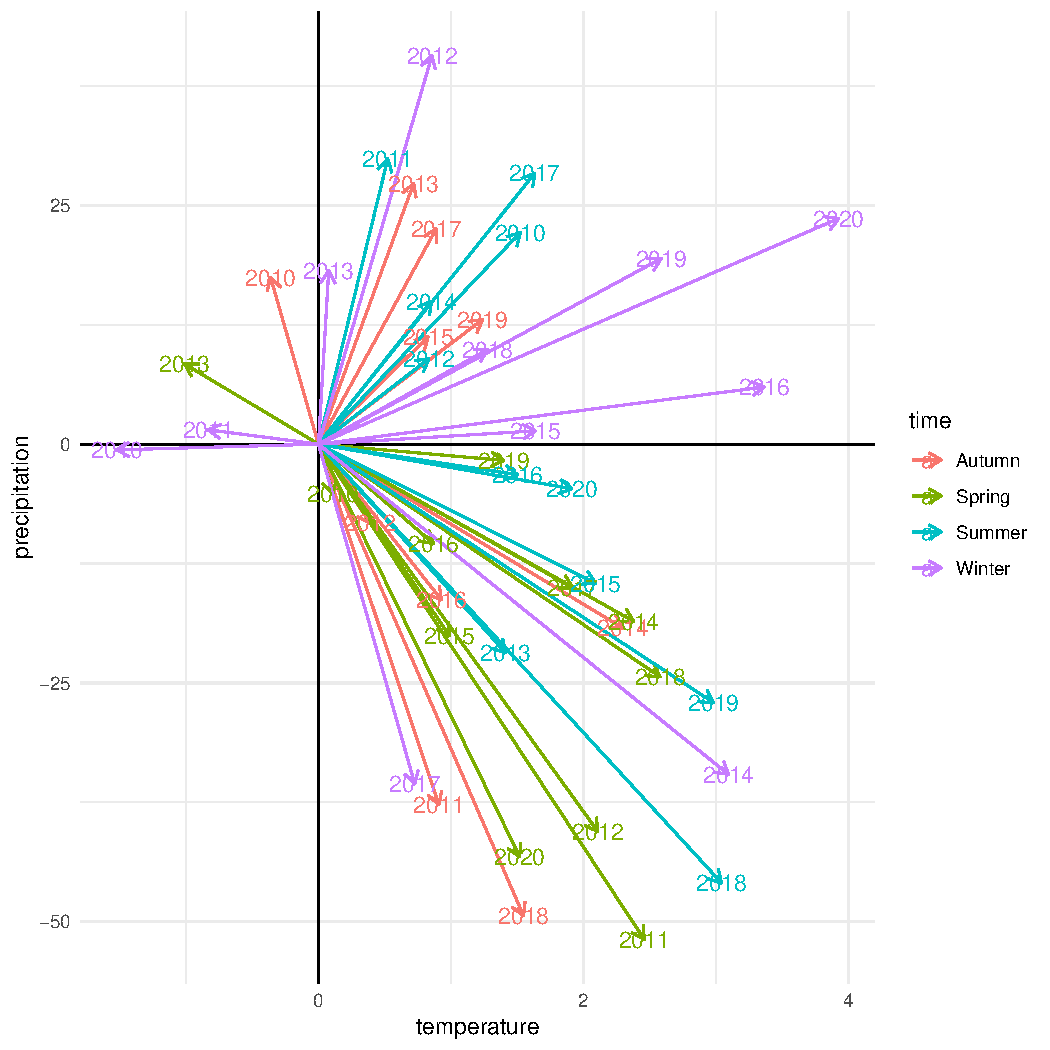
\includegraphics{notebook_files/figure-latex/seasons-1.pdf}

Let's look at where all the years since 1961 are in the plot
(highlighting the most recent years):

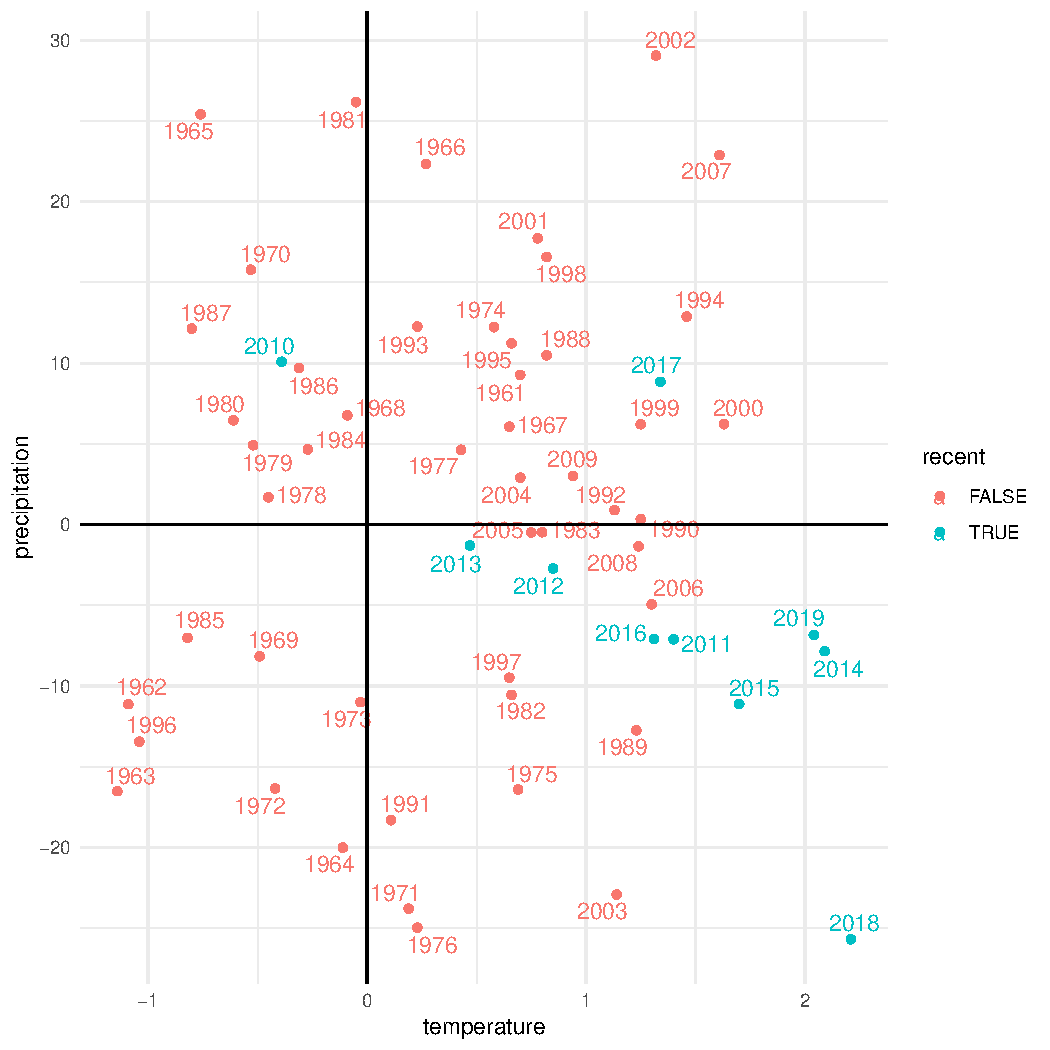
\includegraphics{notebook_files/figure-latex/all_years-1.pdf}

\end{document}
